\chapter{基于客流统计规律的迭代学习模糊控制方法}\label{chap:06}
\setcounter{algorithm}{0} % 重置算法计数器

\section{问题描述}
\label{section2}

本文研究一条具有 $N$ 个车站和 $M$ 列列车（$M > N$）的双线城际铁路线路。列车在两个端点站之间往复运行，并在每个车站停靠以供乘客上下车；抵达端点站后，列车立即折返。该运营模式类似于城市地铁系统，具有发车频率高、停站模式统一、无越行或跨线运行等特点。所有列车均采用全程停站策略，不采用部分交路或跳站运行等方案。

由于站间距较长且服务频率较高，在实际运营中常出现列车数量多于车站数量的情况 \cite{Kang2024}。此外，由于列车运行速度相近，越行在实践中并无必要；若实施越行，则需增设额外基础设施（如越行线），而这类设施在标准双线城际铁路系统中通常并不存在 \cite{Gupta2016}。因此，不考虑越行更符合实际运营规范。

\subsection{城际快铁交通特性}

在城际快铁系统中，列车折返作业通常采用两种方式：站前折返与站后（尾端）折返。前者在同一车站完成下客、上客及方向转换；后者则将下客与上客功能分配至两个相邻车站——在前一站下客，在后一站上客，其折返时间可建模为两站之间的运行时间。尽管存在上述差异，两种情形均可纳入统一的 $M$ 列列车、$N$ 个车站的建模框架中。

本文聚焦于一种环形线路结构，定义如下：

\textbf{环形线路}：指由 $N$ 个车站（编号为 $1$ 至 $N$）组成的闭合线路，其中车站 $N$ 与车站 $1$ 相连，并有 $M$ 列列车（编号为 $1$ 至 $M$）按周期循环运行。各车站的列车发车顺序一致。列车依次停靠各站的顺序为（数字表示列车编号）：
\begin{equation*}
	\{1,2, \cdots, M, 1,2, \cdots, M, 1,2, \cdots\},
\end{equation*}
相应地，车站的访问顺序为：
\begin{equation*}
	\{1,2, \cdots, N, 1,2, \cdots, N, 1,2, \cdots\}.
\end{equation*}

由于高速铁路线路具有环形结构，列车在车站 $1$ 的运行变量与其前序车站 $N$ 密切相关，并受到历史交通状态的影响。

基于此特性，可将实际城际快铁线路抽象为包含 $N$ 个车站的环形模型。通过融合列车运行动态与客流信息，建立描述列车交通行为的动态方程，并据此构建状态空间模型。表 \ref{table1} 汇总了用于刻画列车运行过程的关键变量。

\begin{table}
	\centering
	\caption{变量及其定义}
	\label{table1}
	\begin{tabular}{cp{9cm}}
		\hline
		变量 & 定义 \\
		\hline
		$t_{j}^{i}$ & 列车 $i$ 在车站 $j$ 的实际发车时刻 \\
		$r_{j}^{i}$ & 列车 $i$ 从车站 $j$ 运行至车站 $j+1$ 的实际运行时间 \\
		$s_{j}^{i}$ & 列车 $i$ 在车站 $j$ 的实际停站时间 \\
		$R_{j}$ & 车站 $j$ 至车站 $j+1$ 的计划运行时间 \\
		$u_{j}^{i}$ & 对列车 $i$ 在区间 $[j, j+1]$ 运行时间施加的调度调整量 \\
		$T_{j}^{i}$ & 列车 $i$ 在车站 $j$ 的计划发车时刻 \\
		${w_1}_{j}^{i}$ & 运行时间的扰动项 \\
		${w_2}_{j}^{i}$ & 停站时间的扰动项 \\
		$w_{j}^{i}$ & 总扰动项（$w_{j}^{i} = {w_1}_{j}^{i} + {w_2}_{j+1}^{i}$）\\
		$H$ & 相邻列车之间的发车间隔（追踪间隔）\\
		$\beta$ & 单位乘客平均乘降时间对停站时间的影响系数 \\
		$\phi_{j+1}$ & 车站 $j+1$ 的平均客流量 \\
		$S$ & 列车在车站的最小停站时间 \\
		$x_{j}^{i}$ & 实际发车时刻 $t_j^i$ 与计划发车时刻 $T_j^i$ 的偏差 \\
		\hline
	\end{tabular}
\end{table}

\textbf{符号说明}：本文中，除非另有说明，变量或参数的上标 $i$ 表示列车编号，下标 $j$ 表示车站编号。为体现城际快铁线路的周期性运行特征，上标 $i$ 和下标 $j$ 分别对列车总数 $M$ 和车站总数 $N$ 取模。据此约定，任意两列连续列车可记为 $i$ 与 $i+1$（其中 $1 \leq i \leq M$，且列车 $M$ 之后为列车 $1$）；任意两个连续车站可记为 $j$ 与 $j+1$（其中 $1 \leq j \leq N$，且车站 $1$ 为车站 $N$ 的下一车站）。

\subsection{列车交通流模型方程}

基于城际快铁的运行特性，列车 $i$ 在车站 $j+1$ 的发车时刻可表示为~\cite{VanBreusegem1991}：
\begin{equation}
   t_{j+1}^{i}=t_{j}^{i}+r_{j}^{i}+s_{j+1}^{i} 
\label{eq1}
\end{equation}
其中，$r_{j}^{i}$ 为列车 $i$ 从车站 $j$ 至车站 $j+1$ 的实际运行时间，$s_{j+1}^{i}$ 为列车 $i$ 在车站 $j+1$ 的停站时间。

实际运行时间 $r_{j}^{i}$ 可写为：
\begin{equation}
   r_{j}^{i}=R_{j}+u_{j}^{i}+{w_1}_{j}^{i}
\label{eq2}
\end{equation}
其中，$R_{j}$ 为区间 $[j, j+1]$ 的计划运行时间，$u_{j}^{i}$ 为对该区段施加的运行时间调整量，${w_1}_{j}^{i}$ 为运行时间的不确定性（即运行扰动项）。

在停站时间建模方面，本文考虑当前城际高铁的实际运营场景。近年来，广深城际、京津城际等线路逐步采用类似公交化的灵活运营模式：乘客无需提前订座，可灵活购票，且发车频率更高。然而，这也使得列车在车站的停站时间对客流量更为敏感。具体而言，停站时长主要取决于站台候车乘客数量，而候车人数又与前后列车的发车间隔密切相关~\cite{Kang2024}。综合上述因素，停站时间可建模为：
\begin{equation}
    s_{j+1}^{i}=S+ \beta \phi_{j+1} (t_{j+1}^{i}-t_{j+1}^{i-1})+{w_2}_{j+1}^{i}
\label{eq3}
\end{equation}
其中，$S$ 为最小停站时间，$\beta$ 为单位乘客平均乘降时间对停站时间的影响系数，$\phi_{j+1}$ 为车站 $j+1$ 的平均客流量。当发车间隔增大时，站台积压乘客增多，导致乘降时间延长，进而增加停站时长。此外，${w_2}_{j+1}^{i}$ 表示可能影响停站过程的外部扰动，如突发大客流或操作延误等。

将式 (\ref{eq2}) 与 (\ref{eq3}) 中的两个扰动项合并，得：
\begin{equation}
    w_{j}^{i}={w_1}_{j}^{i}+{w_2}_{j+1}^{i}
\label{eq4}
\end{equation}
其中 $w_{j}^{i}$ 为总扰动项。

将式 (\ref{eq2}) 和 (\ref{eq3}) 代入基本关系式 (\ref{eq1})，并利用式 (\ref{eq4}) 合并扰动项，可得重构后的方程：
\begin{equation}
    (1-\beta \phi_{j+1})t_{j+1}^{i}=t_{j}^{i}-\beta \phi_{j+1}t_{j+1}^{i-1}+S+R_{j}+u_{j}^{i}+w_{j}^{i}
\label{eq5}
\end{equation}

在无扰动的理想运行状态下，城际高铁列车严格按计划时刻表运行。该时刻表由固定发车间隔 $H$ 定义，即：
\begin{equation}
	H=T_{j}^{i+1}- T_{j}^{i}
\label{eq6}
\end{equation}

结合式 (\ref{eq5})，在无控制干预与扰动（即 $u_{j}^{i}=w_{j}^{i}=0$）条件下，计划发车时刻 $T_{j}^{i}$ 应满足：
\begin{equation}
    T_{j+1}^{i}=T_{j}^{i}+\beta \phi_{j+1}H+S+R_{j}
\label{eq7}
\end{equation}

令 $x_{j}^{i}$ 表示实际发车时刻 $t_j^i$ 与计划发车时刻 $T_j^i$ 的偏差，即：
\begin{equation}
    x_{j}^{i}=t_{j}^{i}-T_{j}^{i}  
\label{eq8}
\end{equation}

基于式 \eqref{eq5}、\eqref{eq7} 与 \eqref{eq8}，可通过以下步骤推导新表达式：首先，将式 \eqref{eq7} 中的 $H$ 用式 \eqref{eq6} 替换；其次，将所得方程从式 \eqref{eq5} 中减去，得到差分形式；最后，利用式 \eqref{eq8} 将各项替换为偏差变量 $x_j^i$。最终得到如下方程：
\begin{equation}
    (1-\beta \phi_{j+1})x_{j+1}^{i}+\beta \phi_{j+1}x_{j+1}^{i-1}=x_{j}^{i}+u_{j}^{i}+w_{j}^{i},\quad j\geq1,\ i\geq1
\label{eq9}
\end{equation}

该方程 \eqref{eq9} 亦可改写为：
\begin{equation*}
	x_{j+1}^i=x_j^i-\beta \phi_{j+1}\left(x_{j+1}^{i-1}-x_{j+1}^i\right)+u_j^i+w_j^i
\end{equation*}
显然，该式刻画了列车 $i$ 在车站 $j+1$ 的时刻偏差 $x_{j+1}^i$ 与前序车站 $j$ 的偏差 $x_j^i$ 以及客流因素之间的动态关系。
\label{5.1}

\section{迭代学习预测模型构建}
\label{section3}

根据动态方程 (\ref{eq9})，首先可推导出状态空间模型。结合周期性时刻表特性，第 \ref{3-1} 节建立了批处理形式的状态空间模型；随后，基于预测时域与控制时域，第 \ref{3-2} 节进一步构建了用于模型预测控制（MPC）的迭代学习预测模型。

\subsection{批处理模糊误差模型的建立}
\label{3-1}

本节针对不同列车在不同车站的发车时刻偏差，建立批处理状态空间模型。在提出环形状态空间模型之前，为便于推导，先定义两个矩阵符号。

定义 $H_{1}(a,b)$ 为 $M \times M$ 矩阵，其结构如下：

\begin{equation*}	
	\begin{array}{cccccccc}
		\setlength{\arraycolsep}{0.8mm}
		H_{1}\!\left(N; a_1, a_2, \dots, a_N ; b_1, b_2, \dots, b_{N-1}\right)=\\
		\left[
		\begin{array}{cccc:cccc}
			0&1& & & & & &0 \\
			&\ddots&\ddots& & &0& &\\
			& & &1& & & & \\
			0& & &0&1& & & \\ 
			\hdashline
			0& & &0&a_1&b_1& &0 \\
			& 0&& & &\ddots&\ddots& \\
			&  & && & &a_{N-1}&b_{N-1}\\
			b_N& & &0 & & &0&a_{N}\\
		\end{array}
		\right] \\

		\begin{array}{cc}
			\underbrace{\rule{28mm}{0mm}}_{M-N}&  
			\underbrace{\rule{38mm}{0mm}}_{N}
		\end{array}
	\end{array}
\end{equation*}

定义 $H_{2}(a)$ 为 $M \times N$ 矩阵，其结构如下：

\begin{equation*}
	H_{2}\!\left(N; a_1, a_2, \dots, a_N\right)=
	\begin{array}{ccc}
		\left[
		\begin{array}{ccc}
			 &0& \\
   			\hdashline
			a_1& &0\\ 
			&\ddots& \\
			0& &a_N\\
		\end{array}
		\right]
		&  
		\begin{array}{cc}
			\left.\rule{0mm}{2mm}\right\}M-N \\ \hfill
			\\
			\left.\rule{0mm}{6mm}\right\}N \hfill
		\end{array}
	\end{array}
\end{equation*}

对于每个车站 $j$，分别定义状态向量、控制向量与扰动向量如下：

\begin{gather}
	x_{j}^{i}=\underbrace{\left[x_{j}^{i-M}\; x_{j}^{i-M+1}\; \cdots\; x_{j}^{i-N-1}\right.}_{M-N}\;
	\underbrace{x_{j}^{i-N}\; x_{j-1}^{i-N+1}\; \cdots\; x_{j-N+1}^{i-1}}_{N}]^{\mathrm{T}} \notag \\ 
	U_{j}^{i}=\underbrace{\left[u_{j-1}^{i-N+1}\; u_{j-2}^{i-N+2}\; \cdots\; u_{j-N}^{i}\right]}_{N}^{\mathrm{T}} \notag \\ 
	W_{j}^{i}=\underbrace{\left[w_{j-1}^{i-N+1}\; w_{j-2}^{i-N+2}\; \cdots\; w_{j-N}^{i}\right]}_{N}^{\mathrm{T}}
	\label{eq10}
\end{gather}

本文所引入的状态向量 $x_j^i$ 表示 $M$ 列列车的延误时间。其分量按车站 $j$ 可解释如下：

\begin{enumerate}
    \item 前 $M-N$ 项表示在车站 $j$ 处，编号从 $i-M$ 到 $i-N-1$ 的 $M-N$ 列相邻列车的时刻偏差；
    \item 后 $N$ 项表示 $N$ 列列车的时刻偏差，其特征为上标（列车号）与下标（车站号）之和为同一常数（分别对 $M$ 和 $N$ 取模）。
\end{enumerate}

控制向量 $U_j^i$ 与扰动向量 $W_j^i$ 均为 $N$ 维向量，其元素同样对应于满足“上标与下标之和为常数”的 $N$ 列列车。通过上述定义，可全面刻画列车运行系统的当前状态及所需调整措施，从而在复杂运营场景下实现精确的列车调度优化。类似的状态向量构造方法已在先前研究中被有效采用 \cite{Moaveni2018,Khosrosereshki2021}。

根据式 (\ref{eq10}) 的定义，由基本方程 (\ref{eq9}) 可得如下状态空间方程：

\begin{equation} 
	x_{j}^{i+1}=A x_{j}^{i}+B\left[U_{j}^{i}+W_{j}^{i}\right], \quad j \in\{1,2, \cdots, N\}
	\label{eq11}
\end{equation}
其中
\begin{equation*}
	\begin{gathered}
		A=H_1\!\left(N ;-\frac{z_1}{1-z_1}, \cdots,-\frac{z_N}{1-z_N} ;
		\frac{1}{1-z_1}, \cdots, \frac{1}{1-z_N}\right), \\
		B=H_2\!\left(N ; \frac{1}{1-z_1}, \cdots, \frac{1}{1-z_N}\right).
	\end{gathered}
\end{equation*}

由状态向量定义 (\ref{eq10}) 可知，对于不同车站 $j \in \{1,2,\ldots,N\}$，误差状态空间模型 (\ref{eq11}) 的具体形式虽有差异，但均包含全线各站的客流信息。因此，控制器设计流程对所有模型一致。不失一般性，本文选取某一特定车站 $j_c$（$j_c \in \{1,2,\ldots,N\}$)），并将误差状态空间模型简记为：

\begin{equation} 
	X(i+1)=A X(i)+B\left[U(i)+W(i)\right]
	\label{eq12}
\end{equation}

鉴于实际场景中难以获取足够数据以确定精确的概率分布或切换函数，将乘客需求建模为模糊变量更为合理 \cite{Xu2016,Xu2016a}。本文引入模糊值函数 $\phi_{j+1}$ 以刻画客流量。为逼近式 (10) 所描述的城际高速列车非线性动态调节模型，采用 Takagi–Sugeno (T–S) 模糊建模方法。该方法将局部动态转化为一组线性子系统，从而显著简化控制器设计与稳定性分析过程。

基于 Takagi–Sugeno (T–S) 模糊建模框架 \cite{Tanaka1992}，高速列车重调度的离散时间动态由一组模糊 IF-THEN 规则描述。第 $l$ 条规则表示为：

\textbf{模糊规则 $l$}：若 $\alpha_1$ 为 $M_{l1}$ 且 $\cdots$ 且 $\alpha_N$ 为 $M_{lN}$，则
\begin{equation}
X(k+1) = A_l X(k) + B_l U(k) + D_l W(k), \quad l=1,\ldots,L
\end{equation}
其中，$M_{li}$ ($i=1,2,\ldots,N$) 表示前提变量 $\alpha_i$ 对应的模糊隶属集，$X(k)$ 为状态误差向量，$A_l$、$B_l$ 和 $D_l$ 为第 $l$ 个局部模型对应的常数系统矩阵，$L$ 为模糊规则总数。

通过加权聚合的模糊推理，自动列车调节的 T–S 模糊模型整体行为可表示为：
\begin{equation}
X(i+1) = \sum_{l=1}^{L} h_l(v) \left( A_l X(i) + B_l [U(i) + W(i) ]\right)
\end{equation}
其中 $v = [\alpha_1, \ldots, \alpha_N]$，$h_l(v) = \dfrac{b_l(v)}{\sum_{l=1}^{L} b_l(v)}$，且 $b_l(v) = \prod_{n=1}^{N} M_{ln}(\alpha_n)$。

此处 $M_{ln}(\alpha_i)$ 表示前提变量 $\alpha_i$ 在模糊集 $M_{ln}$ 中的隶属度。由于对所有 $k$ 有 $\sum_{l=1}^{L} b_l(v) > 0$ 且 $b_l(v) \geq 0$，归一化激活强度定义为 $h_l(v) = \dfrac{b_l(v)}{\sum_{l=1}^{L} b_l(v)}$，满足标准凸组合性质：
\[
\sum_{l=1}^{L} h_l(v) = 1, \quad h_l(v) \geq 0, \quad l=1,2,\ldots,L.
\]

本文中，列车运行于环形线路，具有周期性运行特征。为便于分析，将列车运行过程按周期划分为若干“批”（batch），即每一批对应一个运行周期。在此框架下，定义状态向量、扰动向量与控制向量如下：

\begin{equation}
\begin{gathered}
\begin{array}{llll}
X_k(i)=&[x_N^{i-M+(k-1) M} & \cdots & x_N^{i-N-1+(k-1) M}\\
&x_N^{i-N+(k-1) M} & \cdots & x_1^{i-1+(k-1) M}]^{\mathrm{T}}
\end{array} \\
U_k(i)=\left[\begin{array}{lll}
u_{N-1}^{i-N+1+(k-1) M} & \cdots & u_N^{i+(k-1) M}
\end{array}\right]^{\mathrm{T}} \\
W_k(i)=\left[\begin{array}{lll}
w_{N-1}^{i-N+1+(k-1) M} & \cdots & w_N^{i+(k-1) M}
\end{array}\right]^{\mathrm{T}}
\end{gathered}
\label{eq13}
\end{equation}

式 (\ref{eq13}) 中，下标 $k$ 表示批次数，索引 $i$ 表示第 $k$ 批内的决策步。于是，状态空间模型可写为：

\begin{equation}
x_k(i+1) = \sum_{l=1}^{L} h_l(v) \left( A_l x_k(i) + B_l [U_k(i) + W_k(i) ]\right)
\label{eq14}
\end{equation}

考虑有限时间范围 $i \in [0, M]$，将状态向量扩展至整批，可得如下向量形式：

\begin{equation}
\begin{aligned}
& x_k =\left[\begin{array}{llll}
x_k^{\mathrm{T}}(1) & x_k^{\mathrm{T}}(2) & \cdots & x_k^{\mathrm{T}}(M)
\end{array}\right]^{\mathrm{T}} \\
& W_k =\left[\begin{array}{llll}
W_k^{\mathrm{T}}(0) & W_k^{\mathrm{T}}(1) & \cdots & W_k^{\mathrm{T}}(M-1)
\end{array}\right]^{\mathrm{T}} \\
& U_k =\left[\begin{array}{llll}
U_k^{\mathrm{T}}(0) & U_k^{\mathrm{T}}(1) & \cdots & U_k^{\mathrm{T}}(M-1)
\end{array}\right]^{\mathrm{T}}
\end{aligned}
\label{eq15}
\end{equation}

因此，状态空间方程 (\ref{eq14}) 可重写为：

\begin{equation}
\hat{X}_k=\sum_{l=1}^{L} h_l(v) \left( G_l U_k + F_l x_k(0) + G_l W_k \right)
\label{eq16}
\end{equation}
其中 $F_l$ 与 $G_l$ 定义为：
\begin{equation*}
\begin{aligned}
F_l &= 
\begin{bmatrix}
A_l \\
A_l^2 \\
\vdots \\
A_l^M
\end{bmatrix},
& 
G_l &= 
\begin{bmatrix}
B_l & 0 & \cdots & 0 \\
A_l B_l & B_l & \cdots & 0 \\
\vdots & \vdots & \ddots & \vdots \\
A_l^{M-1} B_l & A_l^{M-2} B_l & \cdots & B_l
\end{bmatrix}.
\end{aligned}
\end{equation*}

\subsection{误差预测模型构建}
\label{3-2}

引入模型预测控制（MPC）需考虑两个基本参数：预测时域与控制时域。预测时域指系统未来状态的预测时间跨度，控制时域指每一步优化的未来控制动作数量。通常，控制时域应小于或等于预测时域，以确保控制器仅基于已知状态与输入计算控制量。

为更清晰地刻画相邻两批之间的迭代关系，并正式引入预测与控制时域的概念，将式 (\ref{eq16}) 重写为：

\begin{equation}
\hat{X}_k=x_{k-1}+\sum_{l=1}^{L} h_l(v) \left( G_l \Delta U_k + F_l \Delta x_k(0) + G_l \Delta W_k \right)
\label{eq17}
\end{equation}
其中变量定义为：
\begin{equation*}
\begin{aligned}
& \Delta U_k = U_k - U_{k-1}, \quad
\Delta W_k = W_k - W_{k-1}, \\
& \Delta x_k(0) = x_k(0) - x_{k-1}(0).
\end{aligned}
\end{equation*}

根据式 (\ref{eq17})，在第 $k$ 批的第 $i$ 时刻，对未来 $p$ 步（预测时域为 $p$）的预测可表示为控制时域 $m$ 内的控制量与初始状态的函数：

\begin{equation}
\begin{aligned}
\left[\begin{array}{l}
\hat{X}_k(i+1) \\
\hat{X}_k(i+2) \\
\vdots \\
\hat{X}_k(i+p)
\end{array}\right]
&= \left[\begin{array}{l}
X_{k-1}(i+1) \\
X_{k-1}(i+2) \\
\vdots \\
X_{k-1}(i+p)
\end{array}\right] \\
&\quad + \sum_{l=1}^{L} h_l(v)\left(O_l + J_l + K_l + M_l + N_l\right)
\end{aligned}
\label{eq18}
\end{equation}

式 (\ref{eq18}) 中，$O_l$ 与 $J_l$ 表示强制响应，$K_l$、$M_l$ 与 $N_l$ 表示自由响应。强制响应由外部激励决定：$O_l$ 和 $J_l$ 分别对应预测范围内控制量与扰动量变化的激励作用；自由响应由系统自身特性决定：$K_l$ 与 $M_l$ 分别表示第 $k$ 批在阶段 $i$ 之前的控制量与扰动量的影响，$N_l$ 表示第 $k$ 批初始状态的影响。

具体表达式如下：
\begin{equation*}
O_l = 
\left[\begin{array}{ccc}
B_l & \cdots & 0 \\
\vdots & \ddots & \vdots \\
A_l^{p-1} B_l & \cdots & A_l^{p-m} B_l
\end{array}\right]
\left[\begin{array}{c}
\Delta U_k(i) \\
\Delta U_k(i+1) \\
\vdots \\
\Delta U_k(i+m-1)
\end{array}\right],
\end{equation*}
\begin{equation*}
J_l = 
\left[\begin{array}{ccc}
B_l & \cdots & 0 \\
\vdots & \ddots & \vdots \\
A_l^{p-1} B_l & \cdots & A_l^{p-m} B_l
\end{array}\right]
\left[\begin{array}{c}
\Delta W_k(i) \\
\Delta W_k(i+1) \\
\vdots \\
\Delta W_k(i+m-1)
\end{array}\right],
\end{equation*}
\begin{equation*}
K_l = 
\left[\begin{array}{ccc}
A_l^i B_l & \cdots & A_l B_l \\
\vdots & \ddots & \vdots \\
A_l^{i+p-1} B_l & \cdots & A_l^p B_l
\end{array}\right]
\left[\begin{array}{c}
\Delta U_k(0) \\
\Delta U_k(1) \\
\vdots \\
\Delta U_k(i-1)
\end{array}\right],
\end{equation*}
\begin{equation*}
M_l = 
\left[\begin{array}{ccc}
A_l^i B_l & \cdots & A_l B_l \\
\vdots & \ddots & \vdots \\
A_l^{i+p-1} B_l & \cdots & A_l^p B_l
\end{array}\right]
\left[\begin{array}{c}
\Delta W_k(0) \\
\Delta W_k(1) \\
\vdots \\
\Delta W_k(i-1)
\end{array}\right],
\end{equation*}
\begin{equation*}
N_l = 
\left[\begin{array}{c}
A_l^{i+1} \\
A_l^{i+2} \\
\vdots \\
A_l^{i+p}
\end{array}\right] \Delta x_k(0).
\end{equation*}

根据式 (\ref{eq19}) 的推导（见下文），自由响应项 $K_l$、$M_l$ 与 $N_l$ 可合并为 $F_l \Delta x_k(i)$。最终，迭代学习预测模型可整理为：

\begin{equation}
\begin{aligned}
\hat{X}_k^p(i+1 \mid i) = {}& X_{k-1}^p(i+1) + \sum_{l=1}^{L} h_l(v) \bigl( G_l \Delta U_k^m(i) \\
& + F_l \Delta x_k(i) + G_l \Delta W_k^m(i) \bigr)
\end{aligned}
\label{eq20}
\end{equation}
其中
\begin{equation*}
G_l = 
\begin{bmatrix}
B_l & 0 & \cdots & 0 \\
A_l B_l & B_l & \cdots & 0 \\
\vdots & \vdots & \ddots & \vdots \\
A_l^{p-1} B_l & A_l^{p-2} B_l & \cdots & A_l^{p-m} B_l
\end{bmatrix},
\quad
F_l = 
\begin{bmatrix}
A_l \\ 
A_l^2 \\ 
\vdots \\
A_l^p
\end{bmatrix}.
\end{equation*}

式 (\ref{eq19}) 的推导如下：
\begin{equation}
\begin{aligned}
& A_l^i B_l \Delta U_k(0)+A_l^{i-1} B_l \Delta U_k(1)+\cdots+A_l B_l \Delta U_k(i-1) \\
& + A_l^i B_l \Delta W_k(0)+ A_l^{i-1} B_l \Delta W_k(1)+ \cdots+A_l B_l \Delta W_k(i-1) \\
& + A_l^{i+1} \Delta x_k(0) \\
= & A_l^i\left(A_l \Delta x_k(0)+B_l \Delta U_k(0)+B_l \Delta W_k(0)\right) \\
& + A_l^{i-1} B_l \Delta U_k(1)+\cdots+A_l B_l \Delta U_k(i-1) \\
& + A_l^{i-1} B_l \Delta W_k(1)+ \cdots+A_l B_l \Delta W_k(i-1) \\
= & A_l^i \Delta x_k(1) + A_l^{i-1} B_l \Delta U_k(1) + \cdots + A_l B_l \Delta U_k(i-1) \\
& + A_l^{i-1} B_l \Delta W_k(1) + \cdots + A_l B_l \Delta W_k(i-1) \\
= & A_l \Delta x_k(i).
\end{aligned}
\label{eq19}
\end{equation}

\section{控制器设计与收敛性分析}
\label{section4}

\subsection{迭代学习模型预测控制器设计}

在构建迭代学习模型预测控制器之前，先引入如下矩阵表示：

\begin{equation*}
    H_{3}(a)=
    \begin{array}{ccccccccccc}
    \setlength{\arraycolsep}{1.5mm}
        \left[
        \begin{array}{ccc|ccc}
           0& & & & & 0 \\
           & \ddots& & & & \\
            &  & 0& & & \\ 
            \cline{1-6}
           & & &a& & \\
            & & & &\ddots& \\
           0& & & & &a\\
        \end{array}
        \right]
        &
        \begin{array}{c}
        	 \\
             \left.\rule{0mm}{3.5mm}\right\}M-N  \\ \hfill
             \\
             \\\left.\rule{0mm}{3.5mm}\right\}N \hfill
             \\
        \end{array} \\
        \begin{array}{cc}
            \underbrace{\rule{14mm}{0mm}}_{M-N}&  
            \underbrace{\rule{14mm}{0mm}}_{N}
        \end{array}
    \end{array}
\end{equation*}

基于式 (\ref{eq20}) 所给出的误差预测模型，列车时刻表重调度的目标函数被设计为：在恢复准点性的同时，限制控制量幅值以避免过度调整。该优化问题可表述如下：

\begin{equation}
\begin{aligned}
\min _{\Delta U_k^m(i)} J= & \frac{1}{2}\left\{ \hat{X}_k^p(i+1 \mid i)^{\mathrm{T}} Q \hat{X}_k^p(i+1 \mid i) \right. \\
& \left. + \Delta U_k^m(i)^{\mathrm{T}} R \Delta U_k^m(i) \right\}
\end{aligned}
\label{eq21}
\end{equation}

式 (\ref{eq21}) 中，$Q$ 与 $R$ 为非负对角加权矩阵。第一项旨在恢复计划时刻表，第二项用于惩罚控制量幅值。目标函数采用二次型形式，以联合最小化预测误差与控制输入幅值。该形式不仅兼顾了两项关键性能指标的优化，还保证了目标函数的凸性，从而支持高效可靠的数值求解。

其中权重矩阵定义为：
\begin{equation*}
\begin{aligned}
Q &= 
\left[
\begin{array}{ccc}
H_{3}(q) &        & 0 \\
         & \ddots &   \\
0        &        & H_{3}(q)
\end{array}
\right],
\quad
R = 
\left[
\begin{array}{ccc}
r &        & 0 \\
  & \ddots &   \\
0 &        & r
\end{array}
\right].
\end{aligned}
\end{equation*}

将模型 (\ref{eq20}) 代入目标函数 (\ref{eq21})，并对 $\Delta U_k^m(i)$ 求偏导并令其为零：
\begin{equation}
\frac{\partial J}{\partial \Delta U_k^m(i)}=0
\label{eq22}
\end{equation}

可得最优控制律表达式如下：
\begin{equation}
U_k^m(i)=U_{k-1}^m(i)+\sum_{l=1}^{L} h_l(v)\, H_l \left( E_{k-1}^p(i+1) + F_l \Delta x_k(i) \right)
\label{eq23}
\end{equation}
其中
\begin{equation*}
	H_l=\left(G_l^{\mathrm{T}} Q G_l + R\right)^{-1} G_l^{\mathrm{T}} Q.
\end{equation*}

根据式 (\ref{eq23})，可得学习控制律为：
\begin{equation}
U_k(i)=U_{k-1}(i)+\sum_{l=1}^{L} h_l(v)\, \bar{H}_l \left( x_{k-1}^p(i+1) + F_l \Delta x_k(i) \right)
\label{eq24}
\end{equation}
其中
\begin{equation*}
	\bar{H}_l = \left[\begin{array}{lllll}
		I & 0 & 0 & \cdots & 0
	\end{array}\right] H_l,
\end{equation*}
$I$ 为 $N$ 阶单位矩阵。

系统控制向量由式 (\ref{eq24}) 确定，因此整个问题的计算复杂度主要由该式决定。由于式 (\ref{eq24}) 的总计算复杂度为 $O(N)$ 阶，这一较低的复杂度确保了算法的高效执行，能够很好地满足城际快铁列车实时重调度的需求。

\subsection{基本假设}

为进行收敛性分析，作出以下假设：

\textbf{假设 1}：初始状态设为
\begin{equation}
\label{eq26}
x_k(0)=x_d(0),
\end{equation}
其中 $x_d(0)$ 为期望状态值，$k$ 为迭代次数。

\textbf{假设 2}：相邻两次迭代间的扰动变化有界，其上界为 $b_d$，即
\begin{equation}
\label{eq27}
\sup _{i \in[0, M]}\left\|W_{k+1}(i)-W_k(i)\right\| \leq b_d,
\end{equation}
其中 $W_k(i)$ 与 $W_{k+1}(i)$ 分别为第 $k$ 次与第 $k+1$ 次迭代的扰动向量。

对于城际快铁周期性运行的迭代学习过程，假设 1 可能难以严格满足。当该条件不成立时，可假设初始状态与期望状态的变化为有界量 \cite{Yan2016}。

\subsection{收敛性分析}

基于式 (\ref{eq24})，可得：
\begin{equation}
	\label{eq28}
\Delta U_k(i)=\sum_{l=1}^{L} h_l(v) \left( \bar{H}_l x_{k-1}^p(i+1) + \bar{H}_l F_l \Delta x_k(i) \right).
\end{equation}

结合状态空间模型 (\ref{eq11}) 与相邻批次间的迭代关系，可推导出：
\begin{equation}
\begin{aligned}
\Delta x_k(i) = & \sum_{l=1}^{L} h_l(v) \Big( A_l \Delta x_k(i-1) + B_l \Delta U_k(i-1) + B_l \Delta W_k(i-1) \Big) \\
= & \sum_{l=1}^{L} h_l(v) \left( \sum_{t=0}^{i-1} A_l^t B_l \Delta U_k(i-1-t) + B_l \Delta W_k(i-1) \right).
\end{aligned}
\label{eq29}
\end{equation}

联立式 (\ref{eq28}) 与 (\ref{eq29})，可进一步得到：
\begin{equation}
\begin{aligned}
\Delta U_k(0) = & \sum_{l=1}^{L} h_l(v) \left( \bar{H}_{l,1} x_{k-1}(1) + \bar{H}_{l,2} x_{k-1}(2) + \cdots + \bar{H}_{l,p} x_{k-1}(p) \right), \\
& \vdots \\
\Delta U_k(N-1) = & \sum_{l=1}^{L} h_l(v) \Bigg( \bar{H}_l x_{k-1}^p(N) \\
& - \zeta_{1,l} \sum_{i=0}^{N-2} A_l^i B_l \Delta U_k(N-2-i) - \zeta_{1,l} \sum_{i=0}^{N-2} A_l^i B_l \Delta W_k(N-2-i) \Bigg),
\end{aligned}
\label{eq30}
\end{equation}
其中 $\zeta_{1,l} = \bar{H}_l F_l$。

基于式 (\ref{eq30})，可建立系统误差与控制量之间的如下关系：
\begin{equation}
\Delta U_k = \sum_{l=1}^{L} h_l(v) \left( H_{b,l}^{-1} \left( \bar{H}_l X_{k-1} - H_{d,l} \Delta W_k \right) \right)
\label{eq33}
\end{equation}
其中
\begin{equation*}
H_{b,l} = \left[\begin{array}{cccc}
I & 0 & \cdots & 0 \\
\zeta_{1,l} B_l & I & \cdots & 0 \\
\vdots & \vdots & \ddots & \vdots \\
\zeta_{1,l} A_l^{N-2} B_l & \zeta_{1,l} A_l^{N-3} B_l & \cdots & I
\end{array}\right],
\end{equation*}
\begin{equation*}
H_{d,l} = \left[\begin{array}{cccc}
0 & 0 & \cdots & 0 \\
\zeta_{1,l} \bar{H}_l & 0 & \cdots & 0 \\
\vdots & \vdots & \ddots & \vdots \\
\zeta_{1,l} A_l^{N-2} \bar{H}_l & \zeta_{1,l} A_l^{N-3} \bar{H}_l & \cdots & 0
\end{array}\right],
\end{equation*}
\begin{equation*}
\Delta U_k = \left[\begin{array}{c}
\Delta U_k(0) \\
\Delta U_k(1) \\
\vdots \\
\Delta U_k(N-1)
\end{array}\right],
\quad
X_{k-1} = \left[\begin{array}{c}
x_{k-1}(1) \\
x_{k-1}(2) \\
\vdots \\
x_{k-1}(N)
\end{array}\right].
\end{equation*}

结合式 (\ref{eq17}) 与 (\ref{eq33})，可得：
\begin{equation}
\begin{aligned}
X_k = & X_{k-1} - \sum_{l=1}^{L} h_l(v) \Big( G_l H_{b,l}^{-1} \left( \bar{H}_l X_{k-1} - H_{d,l} \Delta W_k \right) \\
& - F_l \Delta x_k(0) - G_l \Delta W_k \Big).
\end{aligned}
\label{eq34}
\end{equation}

在假设 1（即 $\Delta x_k(0) = 0$）成立的条件下，式 (\ref{eq34}) 可进一步简化为：
\begin{equation}
\begin{aligned}
X_k = & X_{k-1} - \sum_{l=1}^{L} h_l(v) \Big( G_l H_{b,l}^{-1} \bar{H}_l X_{k-1} \\
& + G_l H_{b,l}^{-1} H_{d,l} \Delta W_k - G_l \Delta W_k \Big).
\end{aligned}
\end{equation}

进一步整理得：
\begin{equation}
X_k = \sum_{l=1}^{L} h_l(v) \left( \zeta_{2,l} X_{k-1} + \zeta_{3,l} \Delta W_k \right)
\label{eq36}
\end{equation}
其中
\begin{equation}
\left\{
\begin{array}{l}
\zeta_{2,l} = I - G_l H_{b,l}^{-1} \bar{H}_l, \\
\zeta_{3,l} = G_l H_{b,l}^{-1} H_{d,l} - G_l.
\end{array}
\right.
\label{eq37}
\end{equation}

对式 (\ref{eq36}) 两边取范数，得：
\begin{equation}
\begin{aligned}
\left\|X_k\right\| 
&= \left\| \sum_{l=1}^{L} h_l(v) \left( \zeta_{2,l} X_{k-1} + \zeta_{3,l} \Delta W_k \right) \right\| \\
&\leq \sum_{l=1}^{L} h_l(v) \left( \left\|\zeta_{2,l}\right\| \left\|X_{k-1}\right\| + \left\|\zeta_{3,l}\right\| \left\|\Delta W_k\right\| \right) \\
&\leq \sum_{l=1}^{L} h_l(v) \left( \left\|\zeta_{2,l}\right\| \left\|X_{k-1}\right\| + \left\|\zeta_{3,l}\right\| b_d \right).
\end{aligned}
\label{eq38}
\end{equation}

由式 (\ref{eq38}) 可递推得：
\begin{equation}
\begin{aligned}
\left\|X_k\right\| \leq & \sum_{l=1}^{L} h_l(v) \Big( \left\|\zeta_{2,l}\right\|^{k-1} \left\|X_1\right\| \\
& + \left\|\zeta_{3,l}\right\| b_d \left( 1 + \left\|\zeta_{2,l}\right\| + \cdots + \left\|\zeta_{2,l}\right\|^{k-2} \right) \Big) \\
= & \sum_{l=1}^{L} h_l(v) \left( \left\|\zeta_{2,l}\right\|^{k-1} \left\|X_1\right\| + \frac{ \left\|\zeta_{3,l}\right\| b_d \left( 1 - \left\|\zeta_{2,l}\right\|^{k-1} \right) }{ 1 - \left\|\zeta_{2,l}\right\| } \right).
\end{aligned}
\label{eq39}
\end{equation}

由 $\zeta_{3,l}$ 的定义可知，其为常数矩阵，而 $b_d$ 为相邻迭代间扰动变化的有界值。因此，对式 (\ref{eq39})，当迭代次数 $k \to \infty$ 时，若 $\left\|\zeta_{2,l}\right\| < 1$，则有：
\begin{equation}
	\left\|X_k\right\| \leq \sum_{l=1}^{L} h_l(v) \left( \frac{ \left\|\zeta_{3,l}\right\| b_d }{ 1 - \left\|\zeta_{2,l}\right\| } \right).
\end{equation}

随着迭代次数增加，误差范数 $\left\|X_k\right\|$ 将收敛至有界值 $\sum_{l=1}^{L} h_l(v) \dfrac{ \left\|\zeta_{3,l}\right\| b_d }{ 1 - \left\|\zeta_{2,l}\right\| }$。由此证明了系统的收敛性。所提出的迭代学习模型预测控制方法能够有效保障城际快铁重调度过程的稳定性。

\section{仿真结果}
\label{section5}

在本节中，基于北京至天津城际铁路的实际运营数据进行了数值仿真，涵盖了五大主要客运站：北京南站、武清站、天津站、塘沽站和滨海站。所有仿真实验均在一台高性能服务器上进行，该服务器配备有 Intel Xeon Silver 4210 处理器（2.20 GHz，10 核），80 GB DDR4 内存，并运行 Windows Server 2019 操作系统。仿真平台采用 MATLAB R2023a。

\subsection{仿真参数}

本文参考了从北京至天津城际铁路线收集的工作日全天运营期间（6:00–22:00）的历史进出站客流数据 \cite{zhang2022graph}。客流量全天动态变化，范围在 $[0.1, 0.3]$ 之间。为了提高模型的实际应用性和可扩展性，将客流量建模为时间变化的模糊变量 $\beta(k)$。定义其论域上的六个模糊子集：负大 (NB)、负中 (NM)、负小 (NS)、正小 (PS)、正中 (PM) 和正大 (PB)。NB 的隶属度函数表示当 $\beta(k) = 0.1$ 时具有高可能性，而 NM 对应于 $\beta(k) = 0.3$。NS 反映了 $\beta(k) = 0.2$ 的情况，而 PS 表示 $\beta(k) = 0.15$。PM 表示 $\beta(k) = 0.3$ 时具有高概率，而 PB 表示显著高于基线的偏差，$\beta(k) = 0.1$。

\begin{figure}
	\centering
	
\includegraphics[width=\textwidth]{Img/Ch6/membership.pdf}
	\caption{客流量的隶属度函数}
	\label{fig1:membership}
\end{figure}

采用三角形隶属度函数来刻画这些模糊集，如图~\ref{fig1:membership} 所示。基于历史数据的聚类分析，共提取出 $l = 12$ 条模糊规则用于构建列车调控的非线性动态模型：
\begin{equation}
\begin{array}{r}
x_k(i+1) = \sum_{l=1}^{12} h_l(v) \left( A_l x_k(i) + B_l [U_k(i) + W_k(i) ]\right)
\end{array}
\label{eq14}
\end{equation}
由于 $A_l$、$B_l$ 和 $h_l(v), l =1, 2,... , 12$ 可以通过 (10) 式和图 3 获得，在此不列出以保持论文简洁。

关键仿真参数总结在表~\ref{tab:params} 中。

\begin{table}
\caption{主要仿真参数}
\label{tab:params}
\centering
\small
\begin{tabular}{ll}
\hline
\textbf{参数} & \textbf{值} \\
\hline
列车数量 $M$ & 15 \\
车站数量 $N$ & 5 \\
运营时段 & 6:00--22:00 \\
名义间隔时间 & $H_s = 11.4$\,分钟 \\
客流量 & $\beta(k) \in [0.1, 0.3]$ \\
模糊集合数量 & 6 (NB, NM, NS, PS, PM, PB) \\
模糊规则数量 & $l = 12$ \\
停站时间影响 & $\beta = 0.625$\,分钟/人 \\
加权因子 $q$ & 3 \\
加权因子 $r$ & 1 \\
\hline
\end{tabular}
\end{table}

\subsection{案例 1}

为了验证所提出的迭代学习模糊控制（ILFPC）方法在缓解日常客流波动引起的列车延误方面的有效性，基于一个典型的平日运营场景进行了仿真实验。仿真覆盖整个服务期从 6:00 到 22:00，期间客流量随时间动态变化，表现出明显的早晚高峰模式（早高峰：7:30–9:00；晚高峰：17:30–19:30）。在基准情况下，列车严格按照名义时刻表运行，一旦出现延误则不采取任何控制干预措施。仿真结果如图~\ref{fig2:nocontrol} 所示，其中横轴表示时间，纵轴表示车站编号；每条折线对应一列列车的时空轨迹。可以看出，在早高峰乘客需求的影响下，某些列车经历的初始延误逐渐传播并放大。这一现象表明存在显著的延误传播效应。没有主动调节的情况下，局部扰动迅速演变为系统性的运营不稳定，严重降低准点率和服务质量。

\begin{figure}
	\centering
	
\includegraphics[width=\textwidth]{Img/Ch6/nocontrol.pdf}
	\caption{名义时刻表图（虚线）与实际时刻表（实线）}
	\label{fig2:nocontrol}
\end{figure}

随后，引入了所提出的 ILFPC 方法，在相同的初始条件下对列车运营进行调节。通过将基于模糊逻辑的时间变化客流动态建模与迭代学习框架相结合，ILFPC 控制器生成实时最优调整策略。图~\ref{fig3:mintable} 展示了 ILFPC 策略下的实际列车轨迹。与开环场景相比，受到相同扰动影响的列车能够更快恢复到名义时刻表，延误得到有效限制在局部段落内，不会对后续列车产生连锁影响。所得时刻表显示出显著改进的紧凑性和稳定性。综上所述，实验结果表明，在无控制的情况下，列车延误在现实客流变化下会迅速传播并恶化。相比之下，所提出的 ILFPC 方法通过结合模糊推理的适应性和迭代学习的性能提升能力，实现了卓越的抗干扰效果。它在恢复速度更快、累积延误减少更多以及控制动作更平滑等方面表现出色，从而确保在受随机和时间变化扰动影响的城市轨道交通系统中的稳健可靠运行。

\begin{figure}
	\centering
	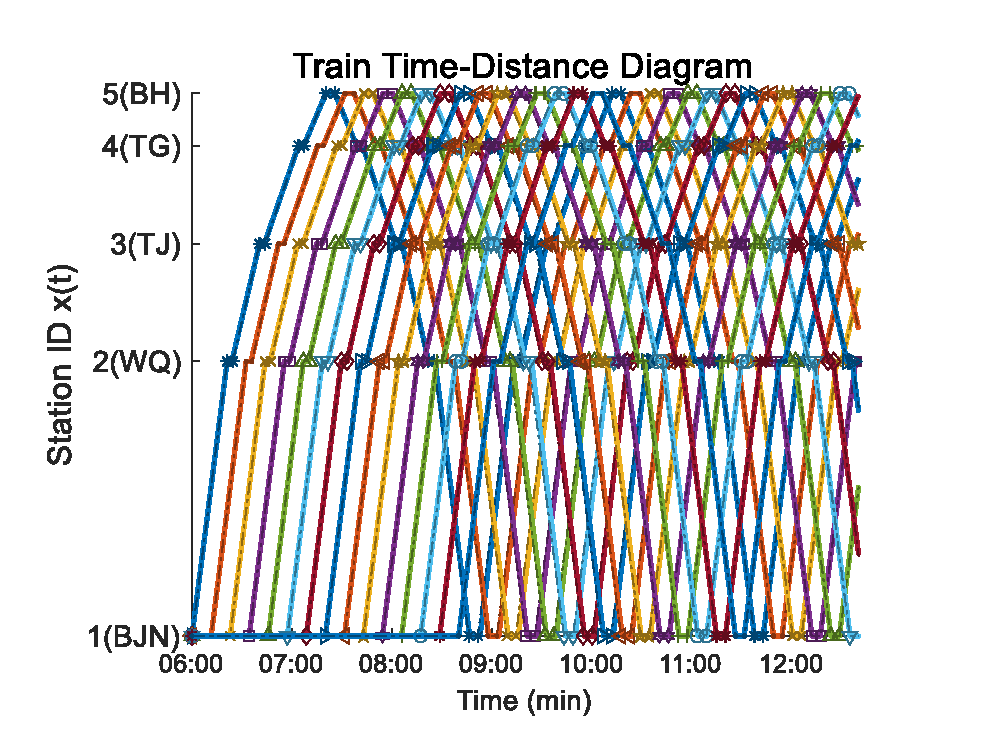
\includegraphics[width=\textwidth]{Img/Ch6/mintimetable.pdf}
	\caption{由迭代模型预测控制方法给出的重调度列车图}
	\label{fig3:mintable}
\end{figure}

\subsection{案例 2}

为了评估所提出的 ILFPC 方法在区域化且持续的客流扰动下的综合调控能力，设计了第二个仿真场景。该场景模拟了在天津站举行大型公共活动，导致整个运营期内（6:00–22:00）上下车乘客数量显著增加。与正常日子相比，该站的客流量增加了约 40\% 至 60\%，导致停车时间延长，成为系统性延误的主要来源。在此背景下，将 ILFPC 方法与迭代学习模型预测控制（IL-MPC）、混合整数规划（MIP）和鲁棒模型预测控制（RMPC）进行了比较，全面评估其在非平稳交通环境中的适应性、实时性能和优化潜力。

\begin{figure}
	\centering
	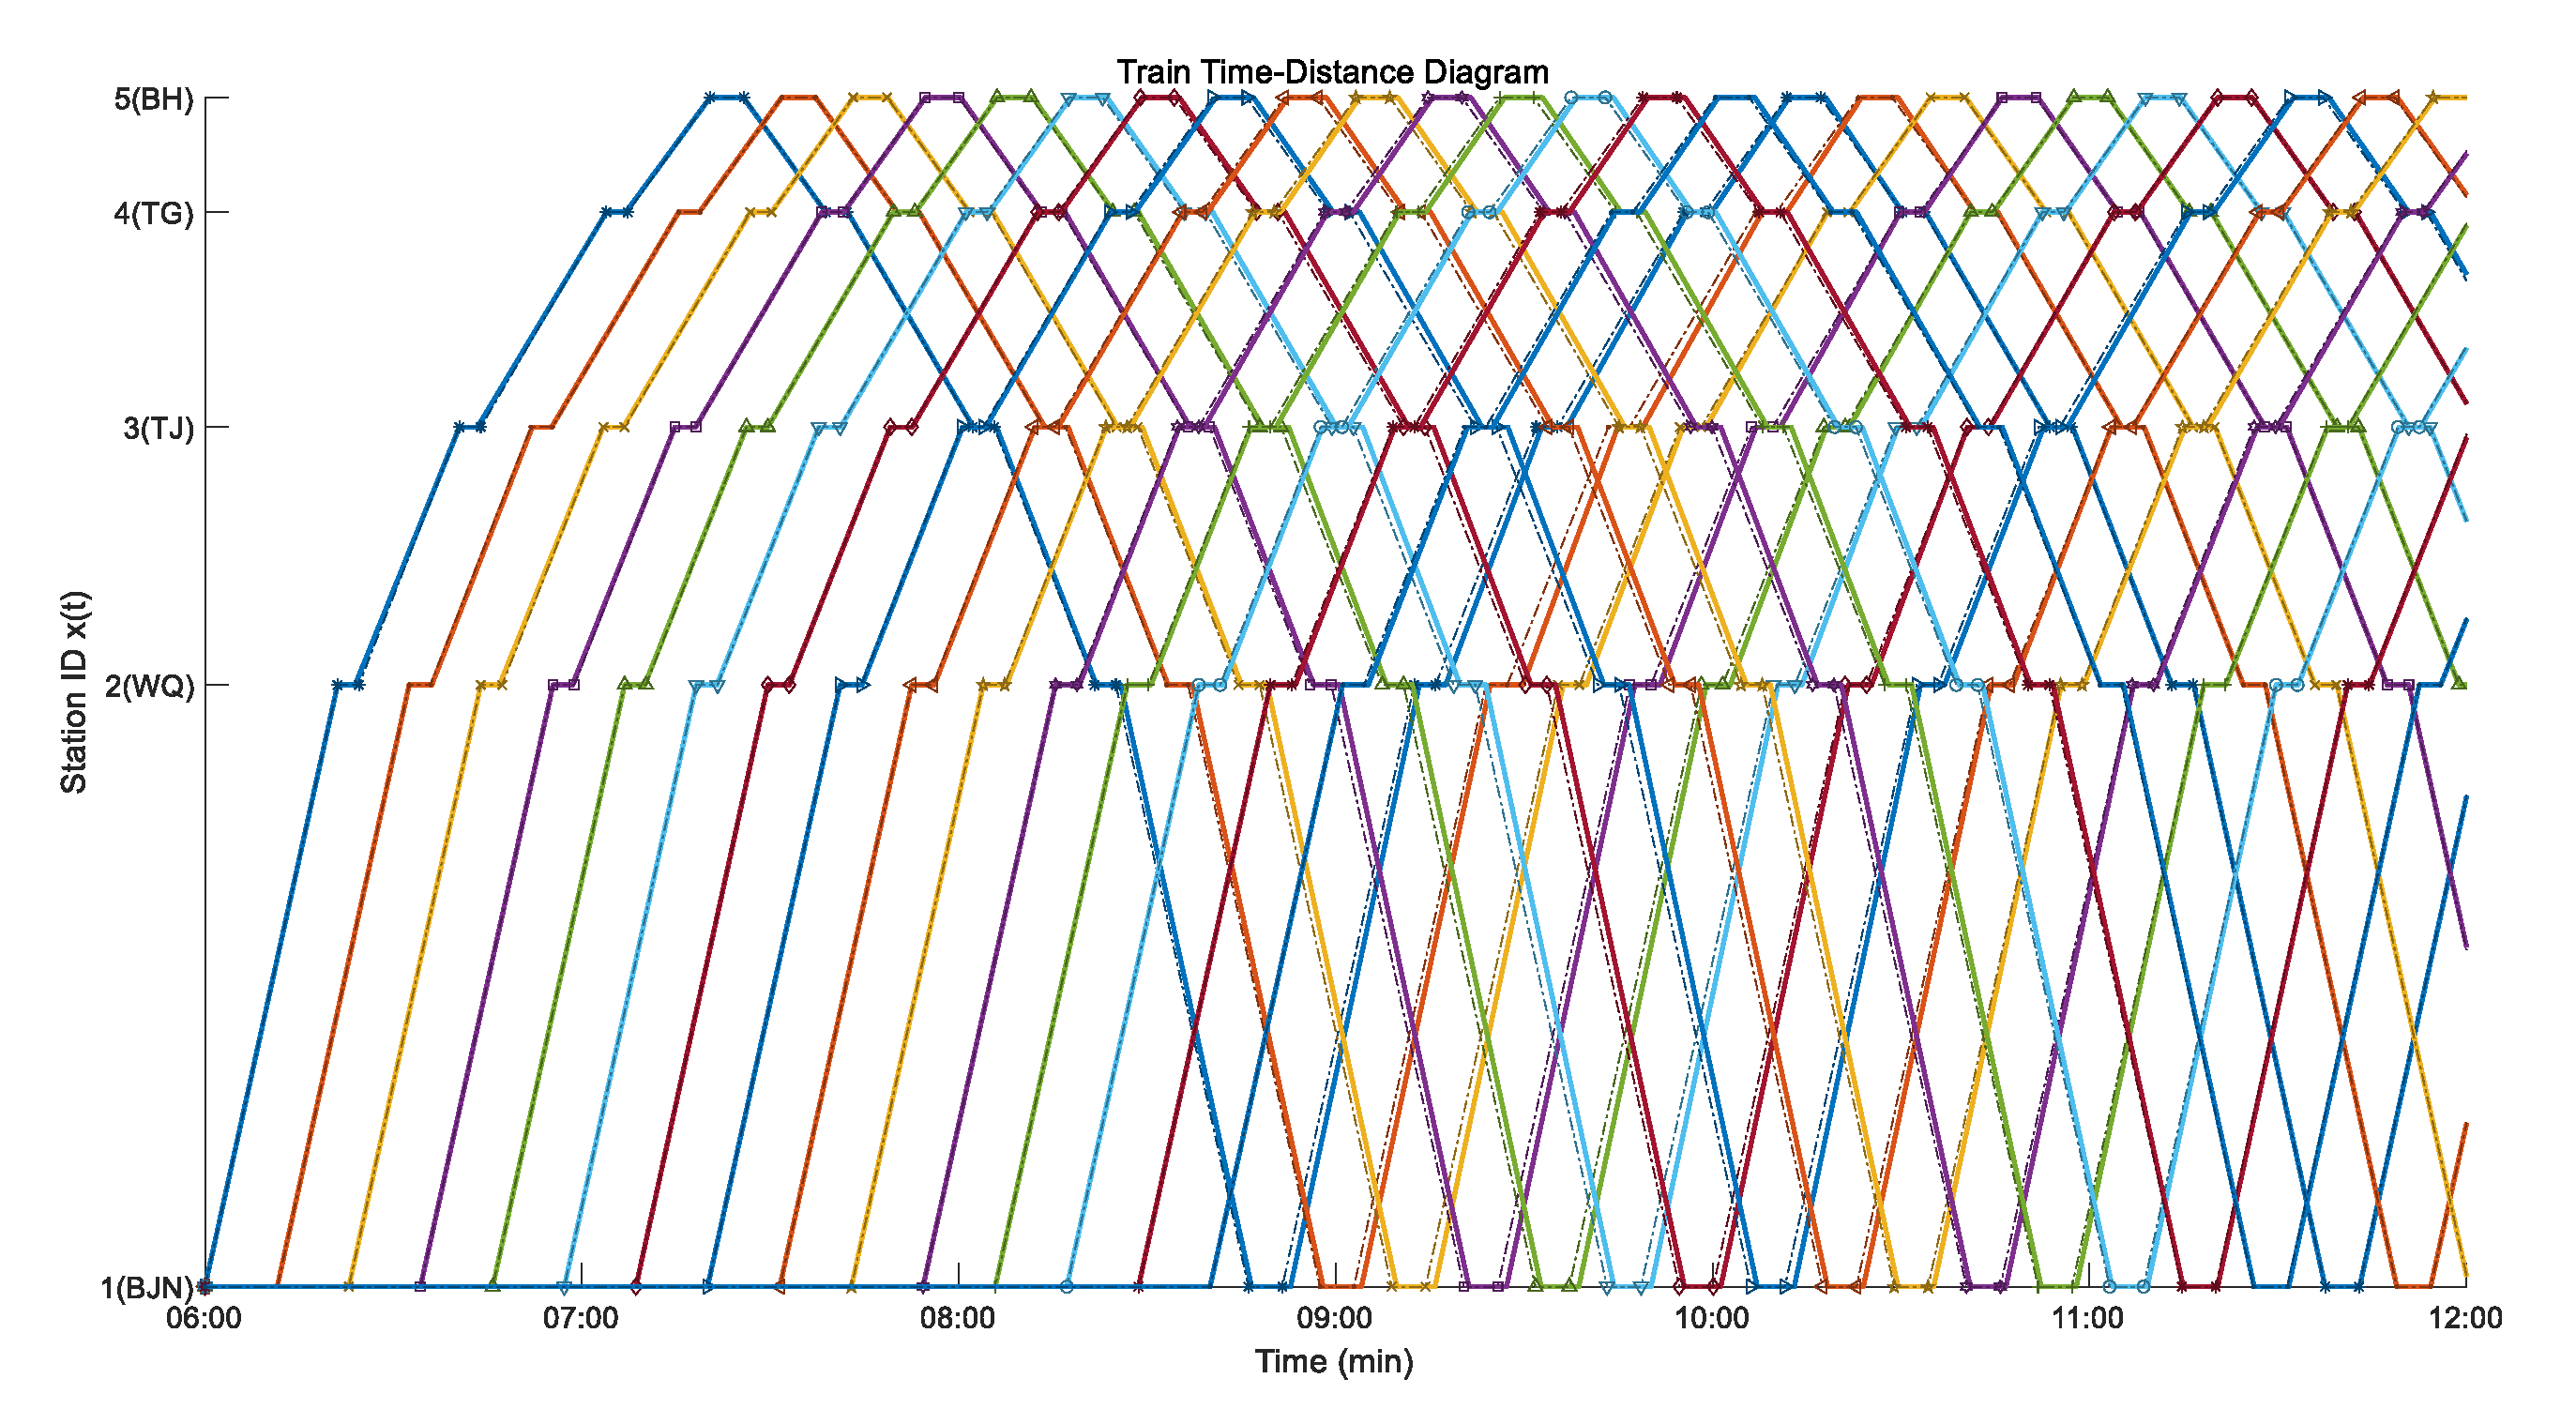
\includegraphics[width=\textwidth]{Img/Ch6/bigtimetable.pdf}
	\caption{由迭代学习模糊预测控制方法给出的重调度列车图}
	\label{fig4:bigtimetable}
\end{figure}

仿真结果显示，所提出的 ILFPC 方法从第一个运行周期就展现出优异的调度性能。如图~\ref{fig4:bigtimetable} 所示，大多数延误在仅仅两个后续站点内即得到恢复，这得益于通过模糊逻辑精确建模的时间变化客流动态。控制器能够根据先验知识快速生成合理的调整策略，有效抑制初始延误的传播。如图~\ref{fig5:contrast} 所示，在第一次运行中，ILFPC 将列车延误限制在 9.2 分钟以内，明显优于 RMPC（19.8 分钟）、MIP（21.8 分钟）和 IL-MPC（16.5 分钟），突显了其强大的鲁棒性和即时控制效果。此外，如图~\ref{fig6:iterative} 所示，ILFPC 方法通过其迭代机制不断整合历史运行数据，自适应地细化控制律参数，在连续周期中实现逐步性能改进。这种进化反映了“每次运行都更好”的特性，这是模糊推理与迭代优化协同作用的结果。

\begin{figure}
	\centering
	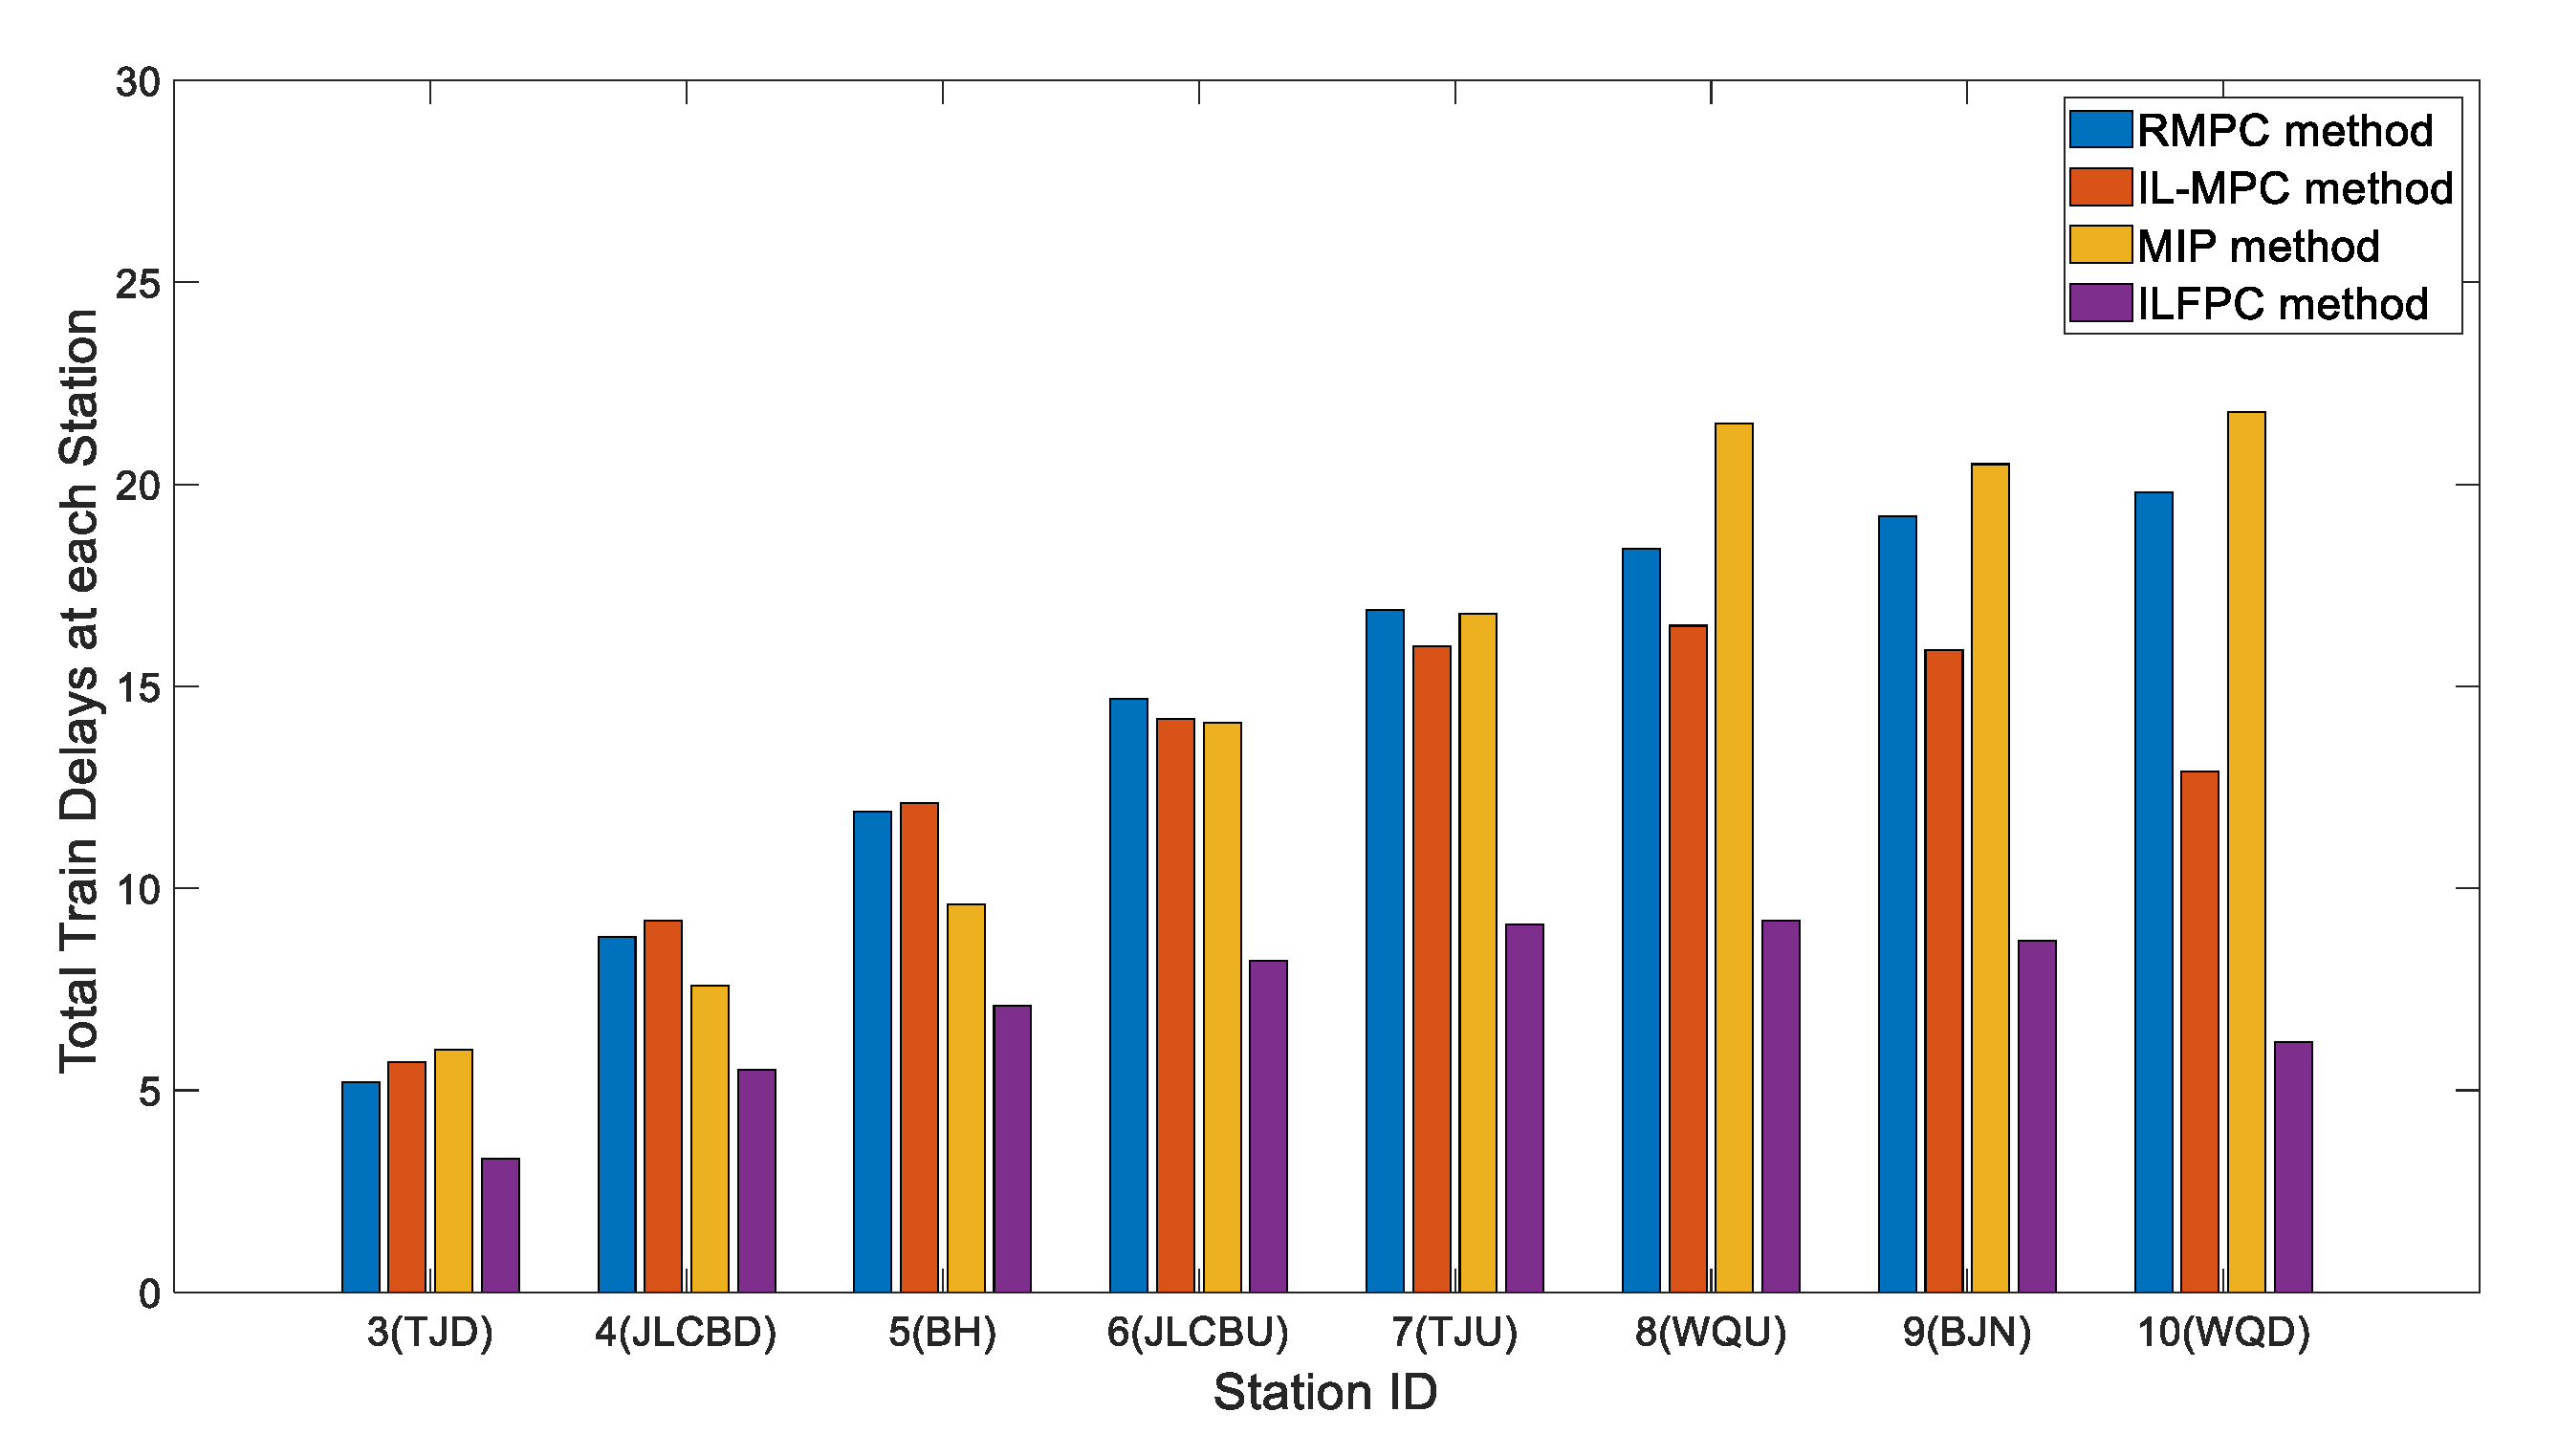
\includegraphics[width=\textwidth]{Img/Ch6/bigdelay.pdf}
	\caption{各站 RMPC、IL-MPC 和 MIP 方法及 ILFPC 的总列车延误时间演化图}
	\label{fig5:contrast}
\end{figure}

\begin{figure}
	\centering
	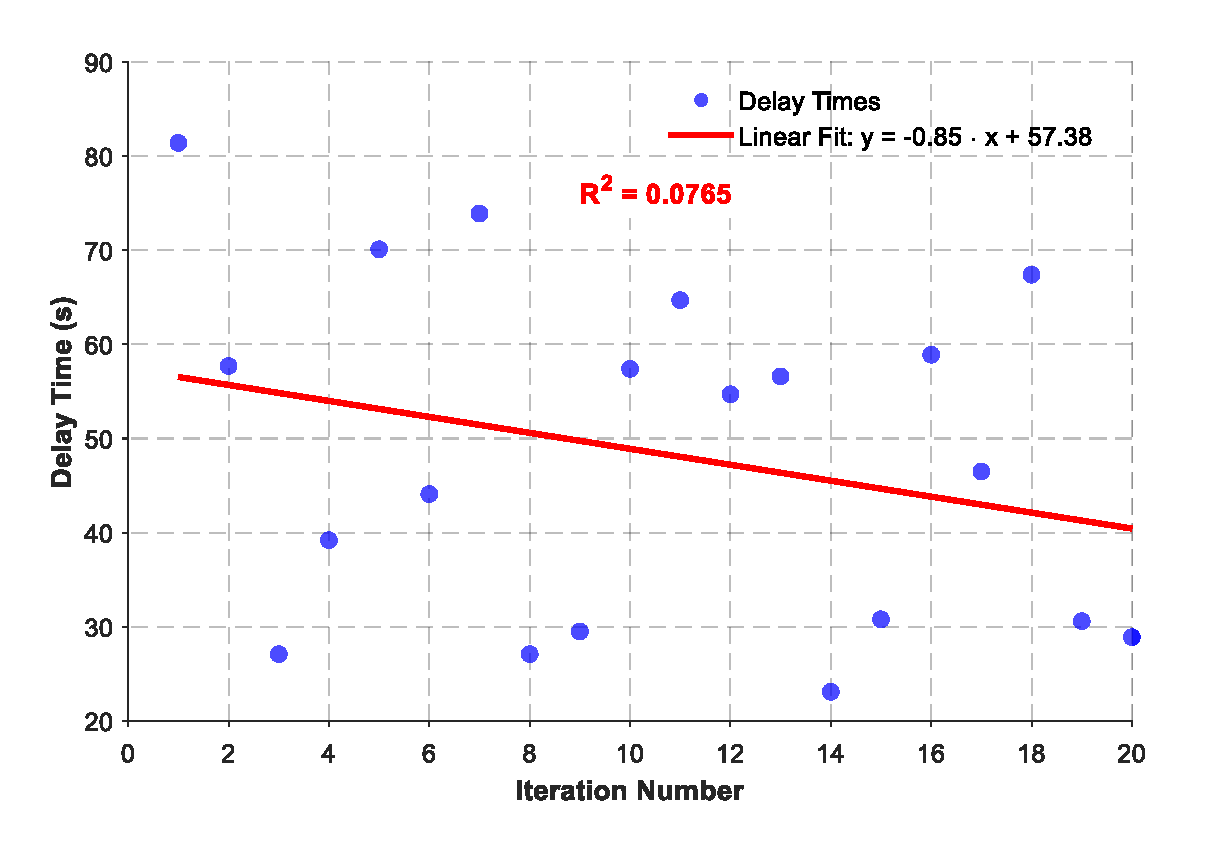
\includegraphics[width=\textwidth]{Img/Ch6/iterative.pdf}
	\caption{总列车延误时间演化图}
	\label{fig6:iterative}
\end{figure}

总之，结果表明，所提出的 ILFPC 方法不仅展示了优越的初始响应——使其具备“即插即用”的实际部署能力，还通过迭代学习不断提高性能。因此，它在处理高速铁路运营中的复杂、时间变化扰动方面展现了巨大潜力，既提供了即时的鲁棒性，又具备长期适应性，适用于未来的智能列车调控系统。

\section{本章小结}
\label{section6}

本章针对城际高速铁路在客流波动等不确定、时变扰动下的列车重调度问题，提出了一种迭代学习模糊预测控制（ILFPC）方法。该方法融合模糊逻辑与迭代学习机制，既能有效刻画由乘客拥堵引起的非线性停站时间变化，又无需依赖精确的系统模型；同时，通过在连续运行周期中不断利用历史信息优化控制策略，实现了“边运行边学习”的自适应调控能力。仿真实验表明，所提 ILFPC 方法在首次运行中即可有效抑制延误传播，并随着迭代次数增加持续降低累积延误，在收敛速度和鲁棒性方面均优于传统反馈控制、模型预测控制及单一迭代学习方法。结果验证了该方法在实际运营不确定性环境下具备良好的应用潜力。未来工作将考虑将其拓展至大规模路网，并与实时客流监测系统集成，以进一步提升调度系统的态势感知与响应能力。